\documentclass[aps,preprint,12pt]{revtex4-2}

% ============================
% Packages
% ============================
\usepackage[T1]{fontenc}
\usepackage[utf8]{inputenc}

\usepackage{amsmath,amssymb,mathtools}
\usepackage{bm}
\usepackage{graphicx}
\usepackage{xcolor}
\usepackage{microtype}
\microtypesetup{expansion=false}

% (Local TeX install has a stub siunitx; keep optional.)
% \usepackage{siunitx}
% \sisetup{per-mode=symbol}
% \DeclareSIUnit\au{a.u.}
% \DeclareSIUnit\angstrom{\text{\AA}}
% \DeclareSIUnit\parsec{pc}

\usepackage{booktabs}
\usepackage{tabularx}

%highlight
% \usepackage{soul}
% Change tracking for Sebas - JW edits in blue
\newcommand{\jwedit}[1]{\textcolor{blue}{#1}}
\newcommand{\jwdelete}[1]{\textcolor{red}{#1}}

\usepackage{tikz}
\usepackage{tikz-cd}
\usetikzlibrary{positioning}

\usepackage[title]{appendix}
%\allowdisplaybreaks[1]

% Bibliography / citations (load before hyperref)
\usepackage{natbib}
\setcitestyle{square, comma, numbers,sort&compress}

% Hyperref must remain late
\usepackage[
  bookmarks=true,
  linktocpage=true,
  pdfpagelabels=true,
  plainpages=false,
  hyperfigures=true,
  colorlinks=true,
  linkcolor=blue,
  citecolor=blue,
  urlcolor=blue
]{hyperref}
\urlstyle{same}

% Theorem environments
\newtheorem{theorem}{Theorem}%[section]
\newtheorem{lemma}[theorem]{Lemma}
\newtheorem{axiom}[theorem]{Axiom}
\newtheorem{proposition}[theorem]{Proposition}
\newtheorem{corollary}[theorem]{Corollary}

% Proof environment (unnumbered; supports optional title)
\newenvironment{proof}[1][Proof]{\par\noindent\textit{#1.}\ }{\hfill\(\square\)\par}

%\theoremstyle{definition}
\newtheorem{definition}[theorem]{Definition}
\newtheorem{remark}[theorem]{Remark}
\newtheorem{observation}[theorem]{Observation}
\newtheorem{example}[theorem]{Example}

\newcommand{\Rec}{\mathrm{Recognition}}
\newcommand{\N}{\mathbb{N}}
\newcommand{\NN}{\mathbb{N}}
\newcommand{\id}{\mathrm{id}}
\newcommand{\Id}{\mathrm{id}}
\newcommand{\Post}{\mathsf{Post}}
\newcommand{\RR}{\mathbb{R}}
% Footnote style
\renewcommand{\thefootnote}{\fnsymbol{footnote}}

%\date{November 2025}

\begin{document}

\title{Coherent Comparison Costs from the d'Alembert Composition Law:\\
Discrete Ledger Structure with a Lean 4 Formalization}

\author{Sebastian Pardo-Guerra}
\email{sebas@recognitionphysics.org}
\affiliation{Recognition Physics Institute}

\author{Megan Simons}
\email{msimons@recognitionphysics.org}
\affiliation{Recognition Physics Institute}

\author{Anil Thapa}
\email{athapa@recognitionphysics.org}
\affiliation{Recognition Physics Institute}

\author{Jonathan Washburn}
\email{washburn@recognitionphysics.org}
\affiliation{Recognition Physics Institute}

\author{Brett Werner}
\email{bwerner@recognitionphysics.org}
\affiliation{Recognition Physics Institute}

\begin{abstract}
We study a calibrated multiplicative d'Alembert functional equation arising from the requirement that comparison costs compose coherently on ratios. The d'Alembert composition law, together with normalization and quadratic calibration at unity, forces the reciprocal cost functional $J(x)=\frac{1}{2}(x+x^{-1})-1$ (Theorem T5; see the companion paper \cite{WashburnZlatanovic2026} for a self-contained proof). We then develop a discrete double-entry ledger model driven by this cost and derive structural consequences including atomic tick updates, closed-chain flux conservation, and scalar potentials on simply connected subgraphs, together with a $2^{d}$-tick periodicity constraint. A Lean~4 formalization of the core derivations is available \cite{Lean4,Mathlib}. We refer to the resulting cost-first framework as \emph{Recognition Science}.
\end{abstract}


\maketitle

\newpage

\section{Introduction}

The question of what minimal structures are required to describe physical phenomena has motivated numerous theoretical frameworks. Traditional approaches begin with spacetime, fields, and equations of motion as primitive concepts. Recognition Science (RS) inverts this perspective by asking: what minimal informational constraints are necessary for recognition to occur, and what mathematical structures emerge from those constraints?

This paper develops the cost-first, ledger-based foundations of Recognition Science: starting from a composition law for comparison costs, we derive a discrete double-entry ledger structure and associated consequences (atomic tick updates, quantization, flux conservation, and discrete scalar potentials), with machine-checked support in Lean~4. A companion paper isolates the keystone uniqueness theorem for the canonical reciprocal cost on $\mathbb{R}_{>0}$ in a self-contained functional-equation treatment.

\subsection{Scope and assumptions}\label{sec:scope}

This manuscript is a mathematical development of a discrete ledger model driven by a reciprocal cost on ratios. All claims of ``necessity'' are \emph{relative} to explicitly stated assumptions (see Definition~\ref{def:relative-necessity}).
\begin{itemize}
    \item \textbf{Input theorem (cost forcing).} We use Theorem~T5 (proved in the companion paper) to fix the canonical reciprocal cost $J$ from the d'Alembert composition law plus normalization and quadratic calibration.
    \item \textbf{Ledger-model assumptions.} The ledger results assume (i) deterministic single-event update semantics $S_{t+1}=U(S_t,e_t)$, (ii) minimality (no intra-tick ordering metadata), (iii) a conservation principle for total balance per tick, (iv) no external sources/sinks, and (v) torsion-free quantized postings in $\delta\mathbb{Z}$.
    \item \textbf{Results established here.} Under these assumptions we derive: atomic tick updates (T2), balanced double-entry postings, quantization of ledger values (T8), cycle flux conservation (T3), and the existence/uniqueness of discrete scalar potentials on connected components (T4), as well as the minimal schedule period bound $T\ge 2^d$ with a Gray-code realization at $d=3$ (T6--T7).
    \item \textbf{Additional hypotheses.} The $D=3$ discussion (Section~\ref{sec:dimension}) combines the $2^d$-period constraint with additional synchronization/linking hypotheses (``gap-45''/golden-angle motivation). It should be read as conditional on those extra hypotheses.
    \item \textbf{Out of scope.} We do not fit data, derive SI numerical constants, or claim physical completeness; links to particular physical models require additional bridging assumptions beyond the present paper.
\end{itemize}

The framework begins with a seemingly abstract question: if we wish to compare two quantities by their ratio, and we require that such comparisons compose coherently, what constraints does this impose? This question leads naturally to the d'Alembert functional equation, which encodes the requirement that comparison costs combine consistently under multiplication and division. Together with normalization and a quadratic calibration at unity, this constraint forces a unique reciprocal cost functional (Theorem~T5).

This paper presents the cost-first ledger framework of Recognition Science, centered on the canonical reciprocal cost functional 
\begin{center}
    $J(x) = \frac{1}{2}(x + x^{-1}) - 1$ 
\end{center}
as the unique solution to the d'Alembert composition law. We then show how ledger structure, discrete time, quantization, conservation laws, potentials, and minimal periodicity constraints follow as consequences of this cost functional together with explicitly stated structural assumptions. The full uniqueness proof of $J$ is deferred to the companion paper; here we treat it as a keystone input and focus on the discrete ledger consequences.

The remainder of this paper is organized as follows. Section~\ref{sec:preliminaries} elucidates the philosophical connection between the cost function and the d'Alembert composition law, explaining why coherent comparison leads to this functional equation. Section~\ref{sec:mathematical} develops the ledger-based framework, using the cost uniqueness theorem (T5) as input and deriving the remaining theorems as consequences. Section~\ref{sec:conclusions} synthesizes the framework and discusses its scope. Appendix~\ref{app:proofs} provides Lean~4 module references for the core theorems.

\section{Motivation: From Coherent Comparison to the d'Alembert Composition Law}\label{sec:preliminaries}

The foundation of Recognition Science rests on a simple but profound insight: if recognition involves comparison, and comparison has a cost, then the requirement that comparisons compose coherently uniquely determines that cost structure. This section elucidates the philosophical and mathematical connection between the idea of coherent comparison and the d'Alembert functional equation.

\subsection{The Primacy of Comparison}

At its most fundamental level, recognition is a relational act: one entity recognizes another. This recognition involves some form of comparison---measuring similarity, difference, or correspondence. In Recognition Science, we formalize this by asking: if we compare two quantities by their ratio $x = a/b$, what ``cost'' or ``defect'' does this comparison incur?

Central to this framework is the idea that the comparison cost $F(x)$ should depend only on the ratio $x$ itself, not on the absolute magnitudes of $a$ and $b$. This reflects the intuition that recognition is fundamentally about \emph{relationships}, not absolute values. Moreover, we require that $F(1) = 0$: when the ratio equals unity, there is perfect balance, no defect, and hence no cost. This will be stated as Axiom A1 (Normalization).

\subsection{Coherent Composition: The d'Alembert Constraint}

The key insight comes from requiring that comparisons compose coherently. Suppose we compare $a$ to $b$, obtaining ratio $x = a/b$ with cost $F(x)$. Then we compare $b$ to $c$, obtaining ratio $y = b/c$ with cost $F(y)$. What should be the cost of comparing $a$ to $c$ directly?

We have two routes to the comparison $a$ to $c$:
\begin{itemize}
    \item \textbf{Direct route:} Compare $a$ to $c$ directly, giving ratio $xy = (a/b)(b/c) = a/c$ with cost $F(xy)$.
    \item \textbf{Composed route:} Combine the two comparisons, which should somehow combine their costs.
\end{itemize}

For the framework to be coherent, these routes should be equivalent. But how do costs combine? The answer lies in the structure of the composition law itself. When we compose comparisons multiplicatively ($xy$), we also have access to the inverse comparison 
\begin{center}
    ($x/y = (a/b)/(b/c) = a/c \cdot c/b = a/b$).
\end{center}
This inverse relationship suggests that costs should combine in a way that respects both the product and the ratio.

The d'Alembert functional equation emerges naturally from this requirement. In its multiplicative form, it states:
\begin{equation}
F(xy) + F(x/y) = 2F(x)F(y) + 2F(x) + 2F(y).
\label{eq:dAlembert-motivation}
\end{equation}

This equation encodes the requirement that the cost of comparing $a$ to $c$ via the composed route ($F(xy) + F(x/y)$) equals the cost of combining the individual comparison costs ($2F(x)F(y) + 2F(x) + 2F(y)$). The specific form of the right-hand side---combining both multiplicative ($F(x)F(y)$) and additive ($F(x) + F(y)$) terms---reflects the dual nature of composition: comparisons can be chained (multiplicative) or compared to each other (additive with interaction). For background on d'Alembert-type functional equations, see e.g.\ \cite{Aczel1966,Kuczma2009}.

This will be Axiom A2 (Composition Law). It is not an arbitrary choice but a necessary condition for coherent comparison. Any alternative composition law would either fail to respect the multiplicative structure of ratios, fail to handle inverse comparisons consistently, or introduce dependencies on absolute magnitudes that violate the relational nature of recognition.

\subsection{Calibration and Uniqueness}

The d'Alembert equation alone does not uniquely determine the cost function. We require one additional constraint to fix the scale. Axiom A3 (Quadratic calibration) specifies that in log coordinates $t=\ln x$, the cost has unit quadratic behavior at unity:
\[
\lim_{t\to 0}\frac{2F(e^t)}{t^2}=1.
\]
If $F$ is twice differentiable at unity, this is equivalent to normalizing the second derivative of the log-lift $G(t)=F(e^t)$ via $G''(0)=1$. This condition fixes the overall scale of the cost.

Together, these three axioms (A1: Normalization, A2: Composition Law, A3: Quadratic calibration) uniquely determine the cost functional. This is the content of Theorem T5, the keystone theorem of Recognition Science. The unique solution is:
\begin{equation}
J(x) = \frac{1}{2}(x + x^{-1}) - 1.
\label{eq:cost-functional}
\end{equation}

Interpretation: coherent comparison together with normalization and calibration eliminates functional-form freedom; under these axioms, the cost is uniquely determined.

\subsection{From Cost to Existence}

Once the cost functional is established, a cascade of implications follows. The cost function $J(x)$ has the property that $J(x) \geq 0$ with equality only when $x = 1$. This immediately yields the \emph{Law of Existence}: a configuration exists (has zero cost) if and only if $x = 1$, i.e., perfect balance.

Moreover, as $x \to 0^+$ or $x \to \infty$, the cost diverges: $J(x) \to \infty$. This means that approaching nothingness (or infinite imbalance) incurs infinite cost. In this way, the classical \emph{Meta-Principle}---``nothing cannot recognize itself''---is not assumed but \emph{derived} as Theorem T1. It reflects the mathematical fact that nothingness is infinitely expensive, not a mysterious pre-logical axiom.

The cost function also exhibits \emph{reciprocity}: $J(x) = J(x^{-1})$ for all $x > 0$. This symmetry forces the double-entry structure of the recognition ledger, as we shall see. Every recognition event must be recorded as a balanced pair, reflecting the symmetric nature of the cost function itself.

The remainder of this paper shows how all structures---discrete time, quantization, conservation laws, potentials, and geometric constraints---emerge as necessary consequences of this unique cost function. 

\section{Mathematical Framework}\label{sec:mathematical}

This section develops the ledger-based framework of Recognition Science. The keystone cost uniqueness theorem (T5) is stated here and proved in the companion paper; we then use it as an input to derive the remaining ledger-structure results under explicit structural assumptions.

The logical structure follows the \emph{cost-first} foundation:
\begin{center}
\textbf{Primitive Axioms (A1--A3)} $\to$ \textbf{T5} (Cost Unique, Keystone) \\
$\to$ \textbf{Law of Existence} $\to$ \textbf{T1} (Meta-Principle) \\
$\to$ \textbf{Ledger Structure} $\to$ \textbf{T2} (Atomic Tick) \\
$\to$ \textbf{T8} (Ledger Units) $\to$ \textbf{T3} (Cycle flux) $\to$ \textbf{T4} (Potential) \\
$\to$ $\phi$ \textbf{selected} $\to$ \textbf{T6--T7} (Minimal period) $\to$ \textbf{D=3}.
\end{center}

\subsection{Notational Convention: Mathematical Necessity}

To ensure precision, we establish the following convention for claims of mathematical necessity:

\begin{definition}[Relative Necessity]
\label{def:relative-necessity}
In this paper, a claim that property $P$ is \emph{mathematically necessary} means: 
$P$ is provable in Lean~4 from the explicitly listed axioms, definitions, and 
structural assumptions stated in this document. Every such claim must reference 
either (i) a theorem with explicitly stated hypotheses, (ii) a lemma with citation 
to the Lean module and exact statement, or (iii) an explicitly labeled assumption 
or axiom.
\end{definition}

This convention ensures that claims of necessity are verifiable and not based on 
hidden premises. When we state that a structure is ``forced'' or ``required,'' we 
will either prove it as a theorem (with explicit hypotheses), state it as an 
explicit assumption, or reference the Lean~4 verification.

\subsection{Taxonomy: Primitive Axioms, Derived Theorems, and Structural Assumptions}

To clarify what is assumed versus what is derived, we classify the foundational 
elements of Recognition Science according to the \emph{cost-first} foundation. The key 
insight: the d'Alembert composition law is \emph{primitive}, and everything else---including 
the Meta--Principle---is derived.

\begin{table}[h]
\centering
\caption{Taxonomy of foundational elements in Recognition Science}
\label{tab:taxonomy}
\begin{tabular}{ll}
\toprule
\textbf{Category} & \textbf{Elements} \\
\midrule
\textbf{Primitive Axioms} & 
A1 (Normalization): $F(1) = 0$ \\
& A2 (Composition Law): $F(xy) + F(x/y) = 2F(x)F(y) + 2F(x) + 2F(y)$ \\
& A3 (Quadratic calibration): $\displaystyle \lim_{t\to 0}\frac{2F(e^t)}{t^2}=1$ \\
\midrule
\textbf{Derived Theorems} & 
T5: Cost Uniqueness: $J(x) = \frac{1}{2}(x + x^{-1}) - 1$ (from A1--A3) \\
& \textbf{Law of Existence}: $x$ exists $\Leftrightarrow$ $J(x) = 0$ \\
& \textbf{T1 (Meta-Principle)}: $J(0^+) \to \infty$ (Nothing costs infinity) \\
& T2: Atomic Tick (from $J$-symmetry + deterministic updates) \\
& T3: Cycle flux conservation (from T8 + double-entry structure) \\
& T4: Potential Uniqueness (from T3 + discrete Poincar\'{e} lemma) \\
& T6: Minimal period $2^d$ (eight ticks for $d=3$) (from T2 + scheduler constraints) \\
& T7: Coverage Lower Bound (from T6 + sampling theory) \\
& T8: Ledger Units (from T2 + discreteness) \\
\midrule
\textbf{Structural Assumptions} & 
Deterministic state-update semantics ($S_{t+1} = U(S_t, e_t)$) \\
& Minimality of ledger structure (no ordering metadata) \\
& Conservation principle: Total balance invariant per tick \\
& Discreteness: No torsion in ledger structure \\
& Lossless interface: Discrete-continuous mapping preserves information \\
\midrule
\textbf{Definitions} & 
Recognition event: $(a,b) \in A \times B$ \\
& Ledger state: $S_t \in \mathcal{S}$ \\
& Tick: Minimal temporal unit for one state update \\
& Posting function: $\Delta(e,t) \in \delta\mathbb{Z}$ \\
& Recognition structure: Directed graph $G=(X,E)$ \\
\bottomrule
\end{tabular}
\end{table}

This taxonomy reflects the \emph{cost-first} foundation: the three primitive axioms (A1--A3) 
force the unique cost functional $J$ (T5), from which the Law of Existence and the 
Meta--Principle are \emph{derived consequences}---not mysterious pre-logical decrees. 
The Meta--Principle becomes a derived boundary consequence: ``Nothing cannot recognize itself'' 
because approaching nothingness incurs infinite cost.

\subsection{The Primitive Foundation: Cost Functional and Uniqueness (T5)}

We begin with the keystone theorem that establishes the unique cost functional. This theorem is the foundation from which all other structures derive.

\textbf{Axiom A1 (Normalization).} The cost at unity is zero: $F(1) = 0$. 
Perfect balance is free.

\textbf{Axiom A2 (Composition Law).} For all $x, y > 0$:
\begin{equation}
F(xy) + F(x/y) = 2F(x)F(y) + 2F(x) + 2F(y).
\label{eq:composition-law}
\end{equation}
This is the d'Alembert functional equation in multiplicative form. It ensures 
that costs combine coherently under multiplicative composition of ratios.

\textbf{Axiom A3 (Quadratic calibration).} In log coordinates $t=\ln x$, define $G(t)=F(e^t)$. We require
\[
\lim_{t\to 0}\frac{2G(t)}{t^2}=\lim_{t\to 0}\frac{2F(e^t)}{t^2}=1.
\]
This fixes the overall scale (and, when $G$ is twice differentiable at $0$, coincides with $G''(0)=1$).

\begin{theorem}[T5: Cost Uniqueness]
\label{thm:cost-unique}
Let $F: \mathbb{R}_{>0} \rightarrow \mathbb{R}$ satisfy:
\begin{enumerate}
    \item \textbf{Normalization (A1):} $F(1) = 0$
    \item \textbf{Composition Law (A2):} $F(xy) + F(x/y) = 2F(x)F(y) + 2F(x) + 2F(y)$
    \item \textbf{Quadratic calibration at unity:} $\displaystyle \lim_{t\to 0}\frac{2F(e^t)}{t^2}=1$
\end{enumerate}
Then, $F$ is uniquely determined:
\begin{equation}
    \label{eq:cost}
    F(x) = \frac{1}{2}(x + x^{-1}) - 1.
\end{equation}
We denote this unique cost functional by $J$.
\end{theorem}

\begin{proof}
See the companion paper \emph{Uniqueness of the Canonical Reciprocal Cost} \cite{WashburnZlatanovic2026} for a self-contained proof. The corresponding Lean statement is \texttt{CostUniqueness.T5\_uniqueness\_complete}.
\end{proof}

The cost functional has the following key properties:
\begin{itemize}
    \item \textbf{Reciprocity:} $J(x) = J(x^{-1})$ for all $x > 0$
    \item \textbf{Non-negativity:} $J(x) \geq 0$ with equality iff $x = 1$
    \item \textbf{Boundary divergence:} $J(x) \to \infty$ as $x \to 0^+$ or $x \to \infty$
\end{itemize}
The boundary divergence is \emph{not assumed}---it is a consequence of the unique 
functional form. This is why the Meta--Principle is derived, not primitive.

\subsubsection{Unique zero-cost configuration (Law of Existence)}

The unique cost functional immediately yields the \emph{Law of Existence}:

\begin{definition}[Zero-cost predicate (RS-existence)]
A configuration $x > 0$ \emph{exists} (in the RS sense) if and only if its defect 
collapses to zero:
\begin{equation}
\text{Exists}(x) \;\Longleftrightarrow\; J(x) = 0.
\end{equation}
\end{definition}

The predicate $\mathrm{Exists}(x)$ introduced above should be understood as a \emph{technical consistency predicate} internal to the Recognition Science (RS) framework, rather than as a claim about ontological presence, representability, or empirical availability. Making this distinction explicit is essential for avoiding conceptual confusion.

Within RS, only the unit configuration $x = 1$ satisfies $\mathrm{Exists}(x)$, corresponding to vanishing defect $J(x)=0$. However, this does \emph{not} imply that configurations with $x \neq 1$ are meaningless, inaccessible, or excluded from the theory. Quite the opposite: recognition events arise precisely when a ratio deviates from unity. Such non-unit configurations carry a strictly positive cost $J(x)>0$, and it is this finite, well-defined cost that renders them \emph{recognizable} and \emph{comparable}. In other words, recognizability is grounded not in zero defect, but in the presence of a quantifiable discrepancy. The function $J(x)$ measures this discrepancy—interpretable as tension, imbalance, or defect—and thereby enables comparison, composition, and iterative processing even away from perfect consistency.

To clarify the logical structure of the framework, it is helpful to separate three related but conceptually distinct notions:
\begin{enumerate}
    \item \textbf{Existence (RS-existence).}  
    This is identified with perfect consistency or zero defect. In the scalar ratio model, it uniquely singles out the unit $x=1$. RS-existence is therefore an equilibrium or consistency predicate: it marks the cost-minimizing identity configuration rather than the totality of admissible states.

    \item \textbf{Recognizability.}  
    A configuration is recognizable whenever a distinction is present, i.e.\ when $x \neq 1$ and hence $J(x)>0$. Such configurations are meaningful inputs to the recognition process precisely because their defect is finite and quantifiable. Recognition operates by \emph{trafficking in nonzero defect}: differences are measured by $J$, composed via the ledger rules, and iterated toward structured outcomes.

    \item \textbf{Equilibrium or stability under iteration.}  
    Truth or actualization in RS is not tied to having zero instantaneous defect, but rather to behavior under repeated recognition. Stable configurations are those that converge toward zero defect under coercive projection, aggregation, or iteration. This is a dynamic, limit-based notion of equilibrium, distinct from the static predicate $\mathrm{Exists}(x)$.
\end{enumerate}

\noindent
Taken together, these distinctions show that RS does not deny the relevance of non-unit configurations; instead, it assigns them a precise operational role. Zero defect marks perfect consistency, while nonzero defect supplies the very substance on which recognition, comparison, and emergent structure depend.

\begin{theorem}[Unique zero-cost configuration]
For $x > 0$: $J(x) = 0 \Leftrightarrow x = 1$. Therefore, unity is the unique 
existent in the RS framework.
\end{theorem}

\begin{proof}
From T5, $J(x) = \frac{1}{2}(x + x^{-1}) - 1$. Setting $J(x) = 0$:
$x + x^{-1} = 2$. Multiplying by $x$: $x^2 - 2x + 1 = 0$, so $(x-1)^2 = 0$, 
giving $x = 1$.

\end{proof}

This is the \emph{Law of Existence} in RS terminology: within the ratio model, the
zero-cost condition $J(x)=0$ has the unique solution $x=1$.

\subsubsection{Properties of the Cost Function}

Near equilibrium ($x=1$), the cost function exhibits quadratic behavior. Let $x=e^\epsilon$ for small $\epsilon$. Then
\begin{equation}
    J(e^\epsilon)=\frac{1}{2}(e^\epsilon + e^{-\epsilon}) - 1 = \cosh(\epsilon)-1 = \frac{\epsilon^2}{2} + \frac{\epsilon^4}{24} + \cdots \approx \frac{1}{2}\epsilon^2,
\end{equation}
reproducing a Euclidean metric in log-space. This local quadratic structure ensures well-behaved optimization near equilibrium.

The cost function has a remarkable self-similar fixed point. Consider the recurrence equation $x_{n+1}=1+1/x_n$, which models self-similar scaling. Fixed points satisfy $x=1+1/x$, yielding the quadratic equation
\[
x^2-x-1=0 \quad \Rightarrow \quad \phi=\frac{1+\sqrt{5}}{2} \approx 1.618.
\]
At $\phi$, the additive (self) and reciprocal (other) components balance. The recognition cost evaluates to
\[
J(\phi)=\frac{1}{2}\left(\phi+\frac{1}{\phi}\right)-1=\phi-\frac{3}{2}\approx 0.118.
\]
By reciprocity, $J(\phi) = J(\phi^{-1})$, so both $\phi$ and its reciprocal $1/\phi \approx 0.618$ lie at the same cost. Thus, $\phi$ marks a natural self-similar scale where the cost function exhibits special symmetry.

\begin{lemma}
If $f(x_1)=f(x_2)$ with $f(x)=x+x^{-1}$, then $x_1=x_2$ or $x_1=1/x_2$.
\end{lemma}

\begin{proof}
From $x_1 + x_1^{-1} = x_2 + x_2^{-1}$, multiply by $x_1 x_2$ and factor to get $(x_1-x_2)(x_1 x_2-1)=0$. Therefore, either $x_1=x_2$ or $x_1 x_2=1$, which implies $x_1=1/x_2$.
\end{proof}

The quantity $J_{\text{bit}}=\ln\phi \approx 0.481$ is a convenient log-scale reference associated with the self-similar fixed point $\phi$. In applications it can be interpreted as a characteristic scale for multiplicative deviations measured in log-coordinates.

\subsection{Boundary divergence (Meta-Principle)}

The Meta--Principle---``Nothing cannot recognize itself''---is not assumed but 
\emph{derived} from the cost functional. Once $J$ is established by T5, the 
Meta--Principle becomes a derived boundary consequence:

\begin{definition}
Given sets \(A\) (recognizer) and \(B\) (recognized), a \emph{recognition event} 
is an ordered pair \((a,b)\in A\times B\). This represents the minimal relational 
structure assumed between recognizer and recognized. We write 
\(\Rec(A,B)=A\times B\) for the set of all recognition events. If either set is 
empty, then \(\Rec(A,B)=\emptyset\).
\end{definition}

\begin{remark}\label{0 and nothing relation}
To connect the ratio model $x=a/b$ to the set-theoretic statement 
\begin{center}
    $\Rec(A,B)=A\times B$,
\end{center}
interpret $a$ and $b$ as nonnegative ``availability/size'' functionals of the underlying domains, e.g. $a:=\mu(A)$ and $b:=\mu(B)$, with $\mu(\emptyset)=0$ and $\mu(\cdot)>0$ for nonempty domains in the intended class.
With this identification, taking $x=a/b$ and holding $b>0$ fixed, the limit $x\to 0^+$ is precisely $\mu(A)\to 0^+$, i.e. the recognizer domain $A$ is depleted toward emptiness/zero-substrate.
In that regime there are no admissible recognition events, since $\mu(A)=0$ corresponds to $A=\emptyset$ (or ``no available elements''), hence $A\times B=\emptyset$ and in particular $\Rec(\emptyset,\emptyset)=\emptyset$.
\end{remark}

\begin{theorem}[T1: Boundary divergence (Meta-Principle)]
\emph{Nothing cannot recognize itself}: 
\begin{center}
    $\Rec(\emptyset,\emptyset)=\emptyset$.
\end{center}

This is a logical tautology (the Cartesian product of empty sets is empty). 
In the ratio model, the corresponding boundary statement is that approaching $x\to 0^+$ incurs infinite cost:
\begin{equation}
\lim_{x \to 0^+} J(x) = +\infty.
\end{equation}
In particular, the $x\to 0^+$ limit lies outside the finite-cost regime of the model.
\end{theorem}

\begin{proof}
From the uniqueness theorem (T5), $J(x) = \frac{1}{2}(x + x^{-1}) - 1$. Moreover, as $x \to 0^+$, the term $x^{-1} \to +\infty$, so $J(x) \to +\infty$. 
Therefore, by Remark \ref{0 and nothing relation}, any configuration approaching ``Nothing'' has unbounded cost.
\end{proof}

The Meta--Principle is no longer a mysterious pre-logical axiom but an 
\emph{derived consistency constraint}: the formalism assigns infinite cost to the $x\to 0^+$ limit via $J(x)\to\infty$, excluding ``nothingness'' configurations from finite-cost recognition dynamics.

\subsection{Single-event updates and atomic ticks}

The atomic-tick principle emerges from the requirement to record recognition events unambiguously. We model recognition dynamics through a \emph{ledger}: a sequential record updated once per tick. When a spatial carrier is assumed later in the paper, we use hypercubic graphs $Q_d$ as a convenient family for analyzing scheduling and coverage constraints; the arguments below do not depend on a specific embedding of the ledger in $\mathbb{R}^d$.

To derive atomicity, we must specify the minimal structural constraints on how the ledger records recognition events. We introduce the following axioms:

\textbf{Axiom 1 (Deterministic State-Update Semantics).}
The ledger state $S_t$ at tick $t$ evolves deterministically according to a function $U: \mathcal{S} \times \mathcal{E} \to \mathcal{S}$, where $\mathcal{S}$ is the state space and $\mathcal{E}$ is the set of recognition events. The state update rule is:
\begin{equation}
    S_{t+1} = U(S_t, e_t),
\end{equation}
where $e_t$ is a \emph{single} recognition event at tick $t$. The function $U$ has domain $(\text{state}, \text{single event})$, not $(\text{state}, \text{set of events})$ or $(\text{state}, \text{sequence of events})$.

\textbf{Axiom 2 (Minimality of Ledger Structure).}
The ledger records only final states at each tick: $S_t$ contains no event-ordering metadata beyond the tick index itself. Recognition events do not commute in general---the order of processing affects the final state for some recognition sequences. Thus, the ledger includes no structure beyond what is necessary for unambiguous recording under Axiom 2. 

Taking the above into consideration, we have the following:

\begin{theorem}[T2: Atomic tick (single-event updates)]
At most one recognition event is processed per tick. There are no concurrent recognitions.
\end{theorem}

Theorem T2 establishes discrete temporal order: time advances in atomic steps. This atomicity follows from Axiom 1 (deterministic state-update semantics): the state transition function $U$ is defined only for single events, so multiple concurrent recognitions in one tick are outside the model. Alternatively, if multiple recognitions could occur in one tick, they would require ordering metadata to determine the state transition (since events do not commute in general), but such metadata is forbidden by Axiom 2 (minimality). Therefore, at most one recognition event per tick.

\subsubsection{Balanced postings (double-entry)}

Theorem T2 establishes \emph{atomicity} but not the posting \emph{structure}. We now show that, under explicit structural assumptions, the double-entry structure (balanced debit--credit pairs) is required by the reciprocity property of the cost function.

The cost function $J(x)$ has the property $J(x) = J(x^{-1})$ (reciprocity), which means that comparing $a$ to $b$ has the same cost as comparing $b$ to $a$. This symmetry forces the double-entry structure: every recognition event must record both the forward comparison (debit) and the inverse comparison (credit), maintaining balance.

\textbf{Structural Assumption: Conservation Principle.}
The total ledger balance is invariant at each tick: if $\mathcal{B}(S_t)$ denotes the total balance (sum over all nodes) of state $S_t$, then $\mathcal{B}(S_{t+1}) = \mathcal{B}(S_t)$ for all $t$.

\textbf{Structural Assumption: No External Sources or Sinks.}
Postings are the only state-changing operations. There are no auxiliary fields, external flows, or hidden variables that can absorb or supply balance.

\begin{proposition}[Double-entry constraint]
Under the following assumptions:
\begin{enumerate}
    \item Atomicity: At most one recognition event per tick (Theorem T2)
    \item Conservation: Total balance is invariant per tick
    \item No external sources/sinks: Postings are the only balance-changing operations
    \item Self-contained state updates: The state $S_{t+1}$ depends only on $S_t$ and the recognition event $e_t$ (Axiom 1)
    \item Cost function reciprocity: $J(x) = J(x^{-1})$ (from T5)
\end{enumerate}
each recognition event must be self-balancing: it must record exactly two postings of equal magnitude and opposite sign, $\pm\delta$ (debit and credit).
\end{proposition}

\begin{proof}
Fix a tick $t$ and suppose a recognition event $e_t$ occurs (if no event occurs, the claim is vacuous). By assumption (2), the total balance must be unchanged: $\mathcal{B}(S_{t+1}) = \mathcal{B}(S_t)$. By assumption (3), the only way to change individual node balances is through postings. By assumption (4), $S_{t+1} = U(S_t, e_t)$ depends only on the current state and the single event.

The reciprocity property (5) from T5 ensures that recognition is symmetric: comparing $a$ to $b$ has the same cost as comparing $b$ to $a$. This symmetry forces the double-entry structure: if node $a$ recognizes node $b$ with posting $+\delta$, then the inverse recognition (node $b$ recognizing node $a$) must have posting $-\delta$ to maintain the symmetry. The minimal structure that satisfies all assumptions is exactly two postings of opposite sign: a debit $-\delta$ and a credit $+\delta$ for some fixed unit $\delta > 0$.

If the recognition event recorded only one posting (say $+\delta$ on one node), then the total balance would change by $+\delta$, violating assumption (2). Similarly, any odd number of postings would create a net imbalance. If it recorded three or more postings with zero net sum, this would be possible in principle, but assumption (4) combined with atomicity requires that the state update be determined solely by the single event $e_t$ and prior state $S_t$, with no auxiliary structure to coordinate multiple postings across different nodes.

\end{proof}

Therefore, under the explicitly stated assumptions and the reciprocity property of the cost function (T5), double-entry accounting (balanced debit--credit pairs) is required. We adopt $\delta > 0$ as the fundamental unit of recognition, with each recognition event recording $+\delta$ (credit) and $-\delta$ (debit) on designated nodes.

To illustrate the preceding ideas, we introduce the following notion and example:

\begin{definition}
    A \textit{recognition structure} is a directed graph $G=(X,E)$ whose edges record elementary recognition relations. We assume $E$ is closed under reversal: if $(x\!\to\!y)\in E$, then $(y\!\to\!x)\in E$.
\end{definition}

\begin{example}[Recognition Structure with Four Nodes]
\label{ex:recognition-structure}
Consider a recognition structure $G=(X,E)$ with four nodes $X=\{a,b,c,d\}$ and directed edges representing recognition relations:
\begin{itemize}
    \item $a \to b$: node $a$ recognizes node $b$
    \item $b \to c$: node $b$ recognizes node $c$
    \item $c \to d$: node $c$ recognizes node $d$
    \item $d \to a$: node $d$ recognizes node $a$
    \item $a \to c$: node $a$ recognizes node $c$
\end{itemize}
This forms a directed graph with a cycle $(a \to b \to c \to d \to a)$ and an additional edge $(a \to c)$ creating a shortcut. At each tick $t$, the ledger assigns postings $\Delta(e,t) \in \delta\mathbb{Z}$ to each edge $e$. For instance, at tick $t=1$, we might have:
\begin{align*}
    \Delta(a \to b, 1) &= +\delta, \\
    \Delta(b \to a, 1) &= -\delta, \\
    \Delta(e, 1) &= 0 \quad \text{for all other edges } e\in E.
\end{align*}
The double-entry rule ensures that for each recognition event, if node $x$ recognizes node $y$ with posting $+\delta$ on edge $(x \to y)$, then node $x$ records a debit and node $y$ records a credit, maintaining balance.
\end{example}

\subsection{Quantized posting units (\texorpdfstring{\bm{$\delta$}}{delta})}

The atomic tick structure with double-entry raises a fundamental question: what is the minimal unit $\delta$? Quantization---the fact that all postings occur in discrete, indivisible units---follows from T2 (atomicity), the requirement $\delta \neq 0$, and the discrete framework. This quantization is established in Theorem T8 (Ledger Units), which proves that for $\delta \neq 0$, the set of ledger increments $\Delta = \{k\delta \mid k \in \mathbb{Z}\}$ forms a cyclic group isomorphic to $\mathbb{Z}$.

Given the double-entry structure derived from T2 and the reciprocity property of the cost function (T5), when a recognition occurs (at most one per tick by T2), it records exactly one balanced pair of magnitude $+\delta$ and $-\delta$. The increment $\delta > 0$ is the fundamental, indivisible quantum of recognition---the smallest positive amount that can be posted on the ledger for any recognition event. This minimal unit is not arbitrary but emerges from the discrete framework's requirement that ledger values be quantized, as formalized in T8.

\subsubsection{Quantization from Atomicity}

The atomic tick structure (T2) together with the requirement that $\delta \neq 0$ and the absence of torsion in the ledger structure immediately implies quantization. This is formalized in the following theorem:

\begin{theorem}[T8: Ledger Units]
For nonzero ledger increment $\delta \neq 0$, the set of all ledger increments
\[
\Delta = \{k \delta \mid k \in \mathbb{Z}\}
\]
forms a cyclic additive group $(\Delta, +)$ isomorphic to $\mathbb{Z}$ under the mapping $k \mapsto k\delta$. 

If the ledger is discrete and $\delta \neq 0$, then all ledger values are integer multiples of $\delta$:
\[
x = n \delta, \qquad n \in \mathbb{Z}
\]
with unique representation (quantization).
\end{theorem}

\begin{proof}
Theorem T2 establishes atomicity: at most one recognition event is processed per tick. Each event records a balanced pair of magnitude $+\delta$ and $-\delta$ for some fundamental increment $\delta > 0$. The discrete nature of the ledger, combined with the requirement that $\delta \neq 0$, implies that all ledger values must be quantized.

Formally, consider the set of all possible ledger increments:
\[
\Delta = \{k\delta \mid k \in \mathbb{Z}\}.
\]
This set forms an additive group under the natural addition operation. The mapping $k \mapsto k\delta$ provides a group homomorphism from $\mathbb{Z}$ to $\Delta$.

Since $\delta \neq 0$ and the ledger structure has no torsion (no finite-order elements other than zero), this homomorphism is injective. Moreover, by construction, every element of $\Delta$ is of the form $k\delta$ for some $k \in \mathbb{Z}$, so the homomorphism is surjective. Therefore, $(\Delta, +) \simeq \mathbb{Z}$ as additive groups.

The uniqueness of representation follows from the absence of torsion: if $k_1\delta = k_2\delta$ for $k_1, k_2 \in \mathbb{Z}$, then $(k_1 - k_2)\delta = 0$. Since $\delta \neq 0$ and there is no torsion, we must have $k_1 = k_2$. Therefore, every ledger value $x$ has a unique representation as $x = n\delta$ for some $n \in \mathbb{Z}$.

This quantization is not an additional assumption but a necessary consequence of T2 (atomicity) combined with the discrete framework and the requirement that $\delta \neq 0$. The algebraic structure ensures that all ledger operations occur in discrete, countable units, providing the foundation for conservation laws and continuity equations.
\end{proof}

Notice that the algebraic structure $(\Delta, +) \simeq \mathbb{Z}$ forbids fractional ledger amounts: every recognition event posts exactly $\pm\delta$ (or integer multiples thereof), all balances are integer multiples of $\delta$, and the isomorphism ensures each amount has a unique integer representation. Each ledger step corresponds to one unit of recognition, guaranteeing unique integer counts for all ledger states. The ledger's arithmetic parallels, at a structural level, how certain physical quantities (e.g., electric charge) appear in discrete units.

\subsection{Cycle flux conservation}

We now derive cycle-level conservation from the double-entry structure (established from the reciprocity property of the cost function and structural assumptions) and quantization (Theorem T8).

\begin{theorem}[T3: Cycle flux conservation]
Under the double-entry ledger structure (balanced debit--credit pairs per recognition event) and quantization (Theorem T8), for every cycle $\gamma$ and tick $t$, the total flux satisfies $\Phi(\gamma, t) = 0$.
\end{theorem}

\begin{proof}
Let $\gamma = (e_1, e_2, \ldots, e_n)$ be a closed cycle. By quantization (T8), all postings are integer multiples of $\delta$: $\Delta(e_i, t) = k_i \delta$ for some $k_i \in \mathbb{Z}$. The cycle flux is $\Phi(\gamma, t) = \sum_{i=1}^n k_i \delta = \delta \sum_{i=1}^n k_i$.

By the double-entry structure (which follows from the reciprocity property of the cost function T5), each recognition event records balanced pairs $\pm\delta$. When we sum postings around a closed cycle, every debit on one edge is matched by a credit on another edge in the cycle (or vice versa). Since the cycle is closed (returns to its starting node), the net balance change around the cycle must be zero: $\sum_{i=1}^n k_i = 0$. Therefore, $\Phi(\gamma, t) = \delta \cdot 0 = 0$.
\end{proof}

Theorem T3 establishes that closed-chain flux is zero under the double-entry ledger structure. This cancellation acts as a discrete analogue of a continuity equation. Under mesh refinement with bounded fluxes, the discrete conservation law recovers the classical continuity equation:
\begin{equation}
   \frac{\partial \rho}{\partial t} + \nabla \cdot \mathbf{J} = 0.
\end{equation}

\textbf{Note on conservation:} The cycle-level conservation (T3) is derived from the structural assumptions: double-entry structure (proven necessary under our assumptions and the reciprocity property of T5) and quantization (T8). The node-level conservation principle (total balance invariant per tick) was stated as a structural assumption earlier. The relationship is: node-level conservation (assumption) + double-entry structure (derived from T5) $\implies$ cycle-level conservation (T3).

\begin{example}[Cycle Flux Conservation]
\label{ex:cycle-flux}
Consider the cycle $\gamma = (a \to b \to c \to d \to a)$ from Example~\ref{ex:recognition-structure}. At a fixed tick $t$, suppose the edge postings are:
\begin{align*}
    \Delta(a \to b, t) &= +2\delta, \\
    \Delta(b \to c, t) &= +\delta, \\
    \Delta(c \to d, t) &= -3\delta, \\
    \Delta(d \to a, t) &= 0.
\end{align*}
The cycle flux is:
\[
\Phi(\gamma, t) = (+2\delta) + (+\delta) + (-3\delta) + (0) = 0.
\]
By Theorem T3, this must always be zero. The double-entry structure ensures balance: if node $a$ recognizes node $b$ with posting $+2\delta$ on edge $(a \to b)$, then $a$ debits $2\delta$ and $b$ credits $2\delta$. Following the cycle, the net change around the loop vanishes, ensuring conservation. If $\Phi(\gamma, t) \neq 0$, it would imply value was created or destroyed, violating the ledger's balance requirement.
\end{example}

\subsection{Discrete potential representation (potential uniqueness)}

Theorem T3 establishes that every closed cycle has zero net flux. This conservation law has profound structural implications: when all cycle fluxes vanish, the ledger postings become path-independent. The sum of postings along any open path depends only on its endpoints, not on the specific route taken. This path independence is the discrete analogue of a curl-free vector field in classical physics, where such fields descend from scalar potentials. The exactness of the RS ledger ensures that recognition patterns arise from underlying scalar potentials.

Formally, the ledger postings form a $1$-cochain on the recognition structure: each oriented edge $e=(x\!\to\!y)$ carries a posting $\Delta(e,t)\in \delta\mathbb{Z}$ at tick $t$. Theorem T3 guarantees that this cochain is closed: for every cycle $\gamma$, the sum $\Phi(\gamma,t)=\sum_{e\in\gamma}\Delta(e,t)$ vanishes. The discrete Poincar\'{e} lemma provides the existence and uniqueness of a potential function that generates these postings.

\begin{definition}
    A \textit{potential function} on a connected component $\mathcal{C}\subseteq X$ is a map $p:\mathcal{C}\to \delta\mathbb{Z}$ such that for each edge $e=(x\!\to\!y)$ in $\mathcal{C}$, the edge difference reproduces the posting: $\Delta(x\!\to\!y,t)=p(y)-p(x)$. This is the standard definition of a discrete gradient.
\end{definition}

\begin{lemma}[Discrete Poincar\'{e} lemma]
Let $G=(X,E)$ be a connected graph and let $\omega:E\to \delta\mathbb{Z}$ be an antisymmetric function: $\omega(y\!\to\!x)=-\omega(x\!\to\!y)$. If the sum of $\omega$ around every cycle is zero, then there exists $p:X\to \delta\mathbb{Z}$ such that $\omega(x\!\to\!y)=p(y)-p(x)$. The function $p$ is unique up to an additive constant.
\end{lemma}

\begin{proof}
Fix a spanning tree $T$ of $G$ and a root $v_0\in X$. For any $v\in X$, there is a unique simple path $P_{v_0\to v}$ in $T$. Define
\[
    p(v):=\sum_{e\in P_{v_0\to v}} \omega(e)\in \delta\mathbb{Z},\quad p(v_0):=0.
\]
For an edge $e=(x\!\to\!y)$ in $T$, concatenating the tree paths shows $p(y)-p(x)=\omega(e)$. If $e\notin T$, adding $e$ to $T$ yields a unique fundamental cycle $C$. By hypothesis $\sum_{f\in C}\omega(f)=0$, and subtracting the tree-edge contributions implies $\omega(e)=p(y)-p(x)$. Thus $\omega=\delta p$. If $\tilde{p}$ also satisfies $\omega=\delta\tilde{p}$, then $\tilde{p}-p$ is constant on $X$.
\end{proof}

Applying the discrete Poincar\'{e} lemma to the ledger postings $\Delta(\cdot,t)$ (which are antisymmetric by the double-entry structure) and using Theorem T3 (which ensures all cycle sums vanish), we obtain the following result:

\begin{theorem}[T4: Potential Uniqueness]
Fix a tick $t$ and a connected component $\mathcal{C}\subseteq X$. Under Theorem T3, there exists a potential
\[
p_t : \mathcal{C} \longrightarrow \delta\mathbb{Z}
\]
such that for each edge $e=(x\!\to\!y)$ in $\mathcal{C}$,
\[
\Delta(e,t) = p_t(y) - p_t(x).
\]
Moreover, $p_t$ is unique up to an additive constant on $\mathcal{C}$.
\end{theorem}

\begin{proof}
Theorem T3 establishes that all cycle fluxes vanish: for every cycle $\gamma$, $\Phi(\gamma, t) = 0$. This means the ledger postings $\Delta(\cdot, t)$ form a closed 1-cochain: the sum around any closed cycle is zero.

The discrete Poincar\'{e} lemma (proved above) provides the key tool: if a 1-cochain $\omega$ is closed (all cycle sums vanish), then there exists a potential function $p$ such that $\omega = \delta p$, where $\delta p$ denotes the discrete gradient (edge differences of $p$).

Applying this to the ledger postings: since $\Delta(\cdot, t)$ is closed by T3, and antisymmetric by the double-entry structure, the discrete Poincar\'{e} lemma guarantees the existence of a potential $p_t$ such that $\Delta(x\!\to\!y, t) = p_t(y) - p_t(x)$ for all edges.

Uniqueness up to an additive constant follows from the fact that if $\tilde{p}_t$ also satisfies $\Delta(x\!\to\!y, t) = \tilde{p}_t(y) - \tilde{p}_t(x)$, then $(\tilde{p}_t - p_t)(y) - (\tilde{p}_t - p_t)(x) = 0$ for all edges, implying $\tilde{p}_t - p_t$ is constant on each connected component.

The proof is constructive: fix a spanning tree, choose a root vertex, and define the potential by summing postings along tree paths. The cycle condition (T3) ensures this definition is consistent for all edges.
\end{proof}

Theorem T4 establishes that every admissible pattern of recognitions arises from a scalar potential. This potential is unique up to an additive constant on each connected component, reflecting the gauge freedom familiar in classical physics. What might appear as a ``force'' or ``balance'' is not an additional construct but a direct outcome of conservation and path-independence, which themselves follow from the double-entry structure forced by the cost function's reciprocity property (T5).

Note that if an edge carries a single posting $\Delta(e,t)=\pm\delta$, then $p_t(y)-p_t(x)=\pm\delta$. More generally, $\Delta(e,t)=k\delta$ implies $p_t(y)-p_t(x)=k\delta$ for some integer $k$.


\begin{example}[Potential Function on a Small Graph]
\label{ex:potential}
Consider the recognition structure from Example~\ref{ex:recognition-structure} with nodes $\{a,b,c,d\}$ and the cycle $(a \to b \to c \to d \to a)$ plus edge $(a \to c)$. At tick $t$, suppose the edge postings are:
\begin{align*}
    \Delta(a \to b, t) &= +2\delta, \\
    \Delta(b \to c, t) &= +\delta, \\
    \Delta(c \to d, t) &= -3\delta, \\
    \Delta(d \to a, t) &= 0, \\
    \Delta(a \to c, t) &= +3\delta.
\end{align*}
Since $\Phi(a \to b \to c \to d \to a, t) = 0$ (as verified in Example~\ref{ex:cycle-flux}), Theorem T4 guarantees a potential exists. Following the constructive proof of the discrete Poincar\'{e} lemma, choose $a$ as the reference vertex and set $p_t(a) = 0$. Then:
\begin{align*}
    p_t(b) &= p_t(a) + \Delta(a \to b, t) = 0 + 2\delta = 2\delta, \\
    p_t(c) &= p_t(b) + \Delta(b \to c, t) = 2\delta + \delta = 3\delta, \\
    p_t(d) &= p_t(c) + \Delta(c \to d, t) = 3\delta + (-3\delta) = 0.
\end{align*}
We verify that $p_t(d) - p_t(a) = 0 - 0 = 0 = \Delta(d \to a, t)$, confirming the cycle closes. For the shortcut edge $(a \to c)$, we check: $p_t(c) - p_t(a) = 3\delta - 0 = 3\delta = \Delta(a \to c, t)$, which is consistent. The potential is unique up to an additive constant: if we had chosen $p_t(a) = k$ instead of $0$, all values would shift by $k$, but the edge differences would remain unchanged.
\end{example}

\subsection{Minimal schedule period \texorpdfstring{$2^d$}{2d}}

Having established atomic single-event updates (Theorem T2), quantization (Theorem T8), and the cost function (Theorem T5), we now examine combinatorial constraints that link a discrete carrier (modeled here by $Q_d$) to discrete time. In particular, we seek lower bounds on the period required to visit all spatial positions under atomic updates.

For the purposes of this section, we treat $d$ as an abstract dimension parameter indexing the hypercube family $Q_d$. A separate (conditional) discussion of selecting $D=3$ is given later.

Thus, the fundamental structure is the $D$-dimensional hypercube $Q_D$, which at $D = 3$ (denoted $Q_3$) provides the minimal cell for ledger-compatible dynamics. The hypercube combinatorics are:

\begin{table}[h]
\centering
\begin{tabular}{lcc}
\toprule
Object & Formula & $D=3$ \\
\midrule
Vertices & $2^D$ & 8 \\
Edges & $D \cdot 2^{D-1}$ & 12 \\
Faces & $2D$ & 6 \\
\bottomrule
\end{tabular}
\caption{Combinatorics of the $D$-cube at $D=3$. The $Q_3$ hypercube has 8 vertices, 12 edges, and 6 faces.}
\end{table}

\subsubsection{Ledger-Compatible Walk Constraints}

Atomic single-event updates impose strict constraints on how recognition events can be scheduled across the spatial network. To characterize the minimal period required to visit all spatial positions, we introduce the concept of a \emph{ledger-compatible walk}: a temporal sequence of recognition events satisfying atomicity and spatial completeness.

Under Theorem T2, each tick processes at most one recognition event. A \emph{ledger-compatible walk} on a $d$-dimensional hypercube $Q_d$ will be modeled as selecting \emph{one} edge traversal per tick (so that spatial completeness is achievable), subject to the following constraints:

\begin{enumerate}
\item \textbf{Atomicity:} At most one event per tick; in this scheduler model we traverse one edge per tick (no concurrent traversals).
    
\item \textbf{Spatial Completeness:} All vertices of $Q_d$ appear at least once per period; the walk is \emph{spatially complete}.
    
\item \textbf{Timestamp Uniqueness:} No vertex appears with multiple timestamps in a single period; each vertex is assigned to a unique tick.
\end{enumerate}

These constraints ensure that the ledger update is both \emph{atomic} (no concurrency) and \emph{complete} (all spatial positions are visited), while maintaining temporal ordering.

As a straightforward consequence, we have the next:

\begin{theorem}[T6: Minimal period \texorpdfstring{$2^d$}{2d} (eight ticks for $d=3$)]\label{thm:T6}
Let $C$ be the vertex set of a $d$-dimensional hypercube $Q_d$, with $|C| = 2^d$, and let $T$ be the scheduler period for a ledger-compatible walk.

\begin{enumerate}
    \item \textbf{(Sufficiency)} If $T \ge 2^d$, then there exists a schedule assigning each vertex of $C$ to a distinct tick, processing one edge traversal per tick without concurrency. For $d = 3$, the Gray code Hamiltonian cycle realizes this minimal period: $000 \to 001 \to 011 \to 010 \to 110 \to 111 \to 101 \to 100 \to 000$.
    
    \item \textbf{(Necessity)} If $T < 2^d$, then $T$ ticks are insufficient to assign a unique tick to each vertex of $C$. By the pigeonhole principle, some tick must carry multiple vertex updates, violating Theorem T2. Hence, no valid ledger-compatible scheduler exists for $T < 2^d$.
\end{enumerate}
\end{theorem}

\begin{proof}
This proof establishes:
\begin{itemize}
    \item Existence of a ledger-compatible walk with period $2^d$ on a $d$-dimensional hypercube $Q_d$
    \item Minimality: no period $T < 2^d$ can satisfy constraints (1)--(3)
    \item Realization via Gray code Hamiltonian cycle (for $d = 3$)
    \item Uniqueness of the minimal period (up to cycle permutation)
\end{itemize}

\textbf{Sufficiency:} For $d = 3$, the Gray code Hamiltonian cycle $000 \to 001 \to 011 \to 010 \to 110 \to 111 \to 101 \to 100 \to 000$ provides a ledger-compatible walk visiting all $2^3 = 8$ vertices exactly once, satisfying all three constraints.

\textbf{Necessity:} By the pigeonhole principle, if $T < 2^d$, then at least two vertices must be assigned to the same tick, violating constraint (3) (timestamp uniqueness). Therefore, $T \ge 2^d$ is necessary.
\end{proof}

Therefore, the minimal period compatible with Theorem T2 for a $d$-dimensional hypercube is exactly
\begin{equation}
    T_{\min} = 2^d.
\end{equation}

For $d = 3$, this yields the eight-tick period: $T_{\min} = 2^3 = 8$ (within the scheduler model above).

Theorem T6 establishes the minimal period for a ledger-compatible walk, but it does not address whether this period is sufficient to distinguish all possible patterns. This leads to a complementary result about coverage:

\begin{theorem}[T7: Coverage Lower Bound]\label{thm:T7}
Let $Q_d$ be a $d$-dimensional hypercube with $2^d$ vertices, and let $T$ be the period of a ledger-compatible walk. If $T < 2^d$, then there exists no surjection from the set of $T$ ticks to the set of all $2^d$ distinct vertex patterns. In other words, $T < 2^d$ cannot cover all possible spatial configurations.
\end{theorem}

\begin{proof}
By the pigeonhole principle, if $T < 2^d$, then at least two distinct vertex patterns must map to the same tick. This violates the requirement that each pattern be uniquely identifiable by its temporal position. The bound $T \ge 2^d$ is necessary for complete pattern coverage, complementing Theorem T6's sufficiency result.

This establishes a sampling-theoretic lower bound analogous to the Nyquist--Shannon theorem: just as a sampling rate of at least twice the highest frequency is required to avoid aliasing, the ledger requires at least $2^d$ ticks to distinguish all $2^d$ vertex patterns without ambiguity.
\end{proof}

Theorem T7 establishes a sampling-theoretic lower bound: just as the Nyquist--Shannon theorem requires a sampling rate of at least twice the highest frequency to avoid aliasing, the ledger requires at least $2^d$ ticks to distinguish all $2^d$ vertex patterns without ambiguity. Together, Theorems T6 and T7 show that $T = 2^d$ is both necessary and sufficient: T6 proves that $T \ge 2^d$ is sufficient for a ledger-compatible walk, while T7 proves that $T < 2^d$ is insufficient for complete pattern coverage. For $D = 3$, this uniquely pins the period to $T = 8$.

\subsection{Conditional dimension selection: $D = 3$}\label{sec:dimension}

We now present a conditional argument selecting $D=3$ under additional hypotheses beyond the scheduling model. Specifically, we combine (i) the $2^D$-tick counting structure with (ii) a ``gap-45'' synchronization criterion and (iii) a linking-based distinguishability requirement.

\begin{theorem}[Conditional dimensional rigidity]
Let $D \in \mathbb{N}$. Assume:
\begin{enumerate}
    \item \textbf{(Gap-45 synchronization hypothesis)} $\mathrm{lcm}(2^D, 45) = 360$.
    \item \textbf{(Linking requirement hypothesis)} dimensions $D<3$ are excluded (e.g.\ because nontrivial linking is required for distinguishability).
\end{enumerate}
Then $D = 3$.
\end{theorem}

\begin{proof}
From $\mathrm{lcm}(2^D,45)=360=8\cdot 45$ we obtain $2^D \mid 8$, hence $D \le 3$.
By the linking requirement hypothesis, $D \ge 3$. Therefore $D=3$.
\end{proof}

\subsubsection{The Linking Argument}

The deeper reason $D = 3$ is special involves \emph{topological linking}:
\begin{itemize}
    \item \textbf{$D = 2$}: Closed curves cannot link irreducibly (Jordan curve theorem). 
    Any two curves can be separated. Linking cost $= 0$.
    \item \textbf{$D = 3$}: Closed curves can link irreducibly (Hopf fibration). 
    The linking number is a topological invariant. Linking cost $= \ln \phi > 0$.
    \item \textbf{$D \geq 4$}: Linked curves can always be unlinked via ambient isotopy. 
    Higher-dimensional ``room'' trivializes linking. Linking cost $\to 0$.
\end{itemize}
Therefore, $D = 3$ is the \emph{unique} dimension with non-trivial linking of closed curves in the classical sense. Interpreting ``distinguishability via linking'' as a model requirement yields a $D=3$ selection under that hypothesis.

The linking penalty $\Delta J = \ln \phi$ connects to the cost functional: it is the 
minimal cost for one recognition event to ``cross'' another in spacetime, establishing 
the fundamental bit-cost of the framework.

\subsubsection{Summary: Three Independent Arguments for $D = 3$}

The conditional $D=3$ selection rests on three independent constraint routes, each sufficient on its own:

\begin{table}[h]
\centering
\caption{Three arguments selecting $D = 3$ (conditional)}
\label{tab:D3forcing}
\begin{tabular}{lll}
\toprule
\textbf{Argument} & \textbf{Constraint} & \textbf{Selects} \\
\midrule
Linking & Non-trivial knot theory & $D = 3$ \\
8-tick & $2^D = 8$ (hypercube counting) & $D = 3$ \\
Gap-45 & $\mathrm{lcm}(2^D, 45) = 360$ & $D = 3$ \\
\bottomrule
\end{tabular}
\end{table}

The convergence of these constraints motivates the following conditional uniqueness statement.

\begin{theorem}[Uniqueness of RS-compatible dimension (conditional)]
There exists a unique RS-compatible dimension:
\begin{equation}
\exists! D \in \mathbb{N} : \text{RSCompatibleDimension}(D).
\end{equation}
That dimension is $D = 3$.

\end{theorem}

\section{Conclusion}\label{sec:conclusions}

This paper develops the cost-first, ledger-based foundations of Recognition Science (RS). The foundation is not a metaphysical decree but a constraint on coherent comparison: the d'Alembert functional equation. The canonical reciprocal cost functional
$J(x) = \frac{1}{2}(x + x^{-1}) - 1$
is \emph{uniquely forced} by the d'Alembert composition law together with normalization and quadratic calibration (Theorem~T5; see the companion paper for a self-contained proof). From this keystone theorem, the remaining structures follow under the stated structural assumptions:

\begin{itemize}
\item The \textbf{Law of Existence}: a configuration exists iff $J(x) = 0$, which holds 
uniquely at $x = 1$.
\item The \textbf{Meta-Principle} (T1): ``Nothing cannot recognize itself'' is \emph{derived}---it 
reflects the mathematical fact that $J(0^+) \to \infty$.
\item The \textbf{ledger structure}: $J$-symmetry ($J(x) = J(x^{-1})$) forces double-entry 
bookkeeping.
\item \textbf{Discrete time} (T2), \textbf{quantized units} (T8), \textbf{cycle flux conservation} (T3), 
\textbf{scalar potentials} (T4), and the \textbf{minimal period constraint} (T6--T7) follow from the cost function and structural assumptions.
\item The \textbf{golden ratio} $\phi$: self-similarity in a discrete ledger uniquely selects 
$\phi$ as the scaling factor.
\item \textbf{Three-dimensional space} ($D = 3$): a conditional selection argument is given under additional synchronization/linking hypotheses (Section~\ref{sec:dimension}).
\end{itemize}

The cost-first foundation is the conceptual core of Recognition Science. In this framework, the Meta-Principle is not introduced as a pre-logical or metaphysical postulate; it follows from the boundary behavior of the unique cost functional, namely $J(x)\to\infty$ as $x\to 0^+$ or $x\to\infty$. In the ledger model, this divergence acts as a consistency barrier: the ``nothing'' limit is not reachable within finite cost, so the corresponding principle is derived within the formalism.

Recognition Science (RS) provides a \emph{structural framework} in which discrete outcomes arise as consequences of an explicit cost-and-ledger formalism rather than as phenomenological inputs or approximations. All discrete statements produced within RS are intended to be supported by machine-checked proofs implemented in Lean~4, subject to the stated assumptions and the scope limitations noted in Section~\ref{sec:scope}.

Within its explicitly stated domain of validity, RS functions as a \emph{unifying organizational framework} for dynamical theories. It does not modify, extend, or replace existing physical laws by introducing new degrees of freedom or interaction terms. Instead, it constrains the space of admissible effective theories by identifying the unique cost-minimizing structure compatible with recognition, balance, and composability. Familiar dynamical frameworks—classical, quantum, and continuum descriptions—emerge as effective realizations of this underlying structure, appearing not by construction but by necessity.

Having established the cost functional, its uniqueness under the stated axioms, and the hierarchy of derived ledger structures, we thereby provide a rigorous foundation for further applications. The present work focuses on the forcing chain up through discrete ledger consequences (T1--T8) and their formal verification; quantitative connections to particular physical models or constants, when desired, require additional bridging assumptions and are outside the scope of this paper.


\begin{thebibliography}{99}

\bibitem{Aczel1966}
J.~Acz\'{e}l,
\emph{Lectures on Functional Equations and Their Applications}.
Academic Press, 1966.

\bibitem{Kuczma2009}
M.~Kuczma,
\emph{An Introduction to the Theory of Functional Equations and Inequalities}, 2nd ed.
Birkh\"{a}user, 2009.

\bibitem{Lean4}
L.~de Moura and contributors,
\emph{Lean 4 Theorem Prover}.
\url{https://leanprover.github.io/}.

\bibitem{Mathlib}
The mathlib community,
\emph{Mathlib: the Lean mathematical library}.
\url{https://github.com/leanprover-community/mathlib4}.

\bibitem{WashburnZlatanovic2026}
J.~Washburn and M.~Zlatanovi\'{c},
\emph{Uniqueness of the Canonical Reciprocal Cost}.
Preprint, 2026.

\end{thebibliography}

\begin{appendix}

\section{Proofs of Core Theorems}\label{app:proofs}

All theorems T1--T8 have corresponding Lean~4 statements in the \texttt{IndisputableMonolith} repository, with machine-checkable proofs for the core forcing chain. We will provide a public archive with version control, build instructions, and a fixed commit hash corresponding to the version referenced by this manuscript.

\textbf{Note on reproducibility:} For proper scientific reproducibility, the archive will include: (i) a public repository URL (e.g., GitHub/GitLab) with version control, (ii) a specific commit hash corresponding to the verification status reported here, (iii) build instructions and dependency specifications (e.g., \texttt{lean-toolchain} and \texttt{lakefile.lean}), (iv) continuous integration (CI) configuration to verify builds, and (v) documentation for reproducing the verification.

\subsection{Logic Decomposition Flow (Cost-First Foundation)}

The dependency structure follows the \emph{cost-first foundation}. T5 (Cost Uniqueness) 
is the \emph{keystone theorem}, from which everything else derives.

\begin{figure}[h]
\centering
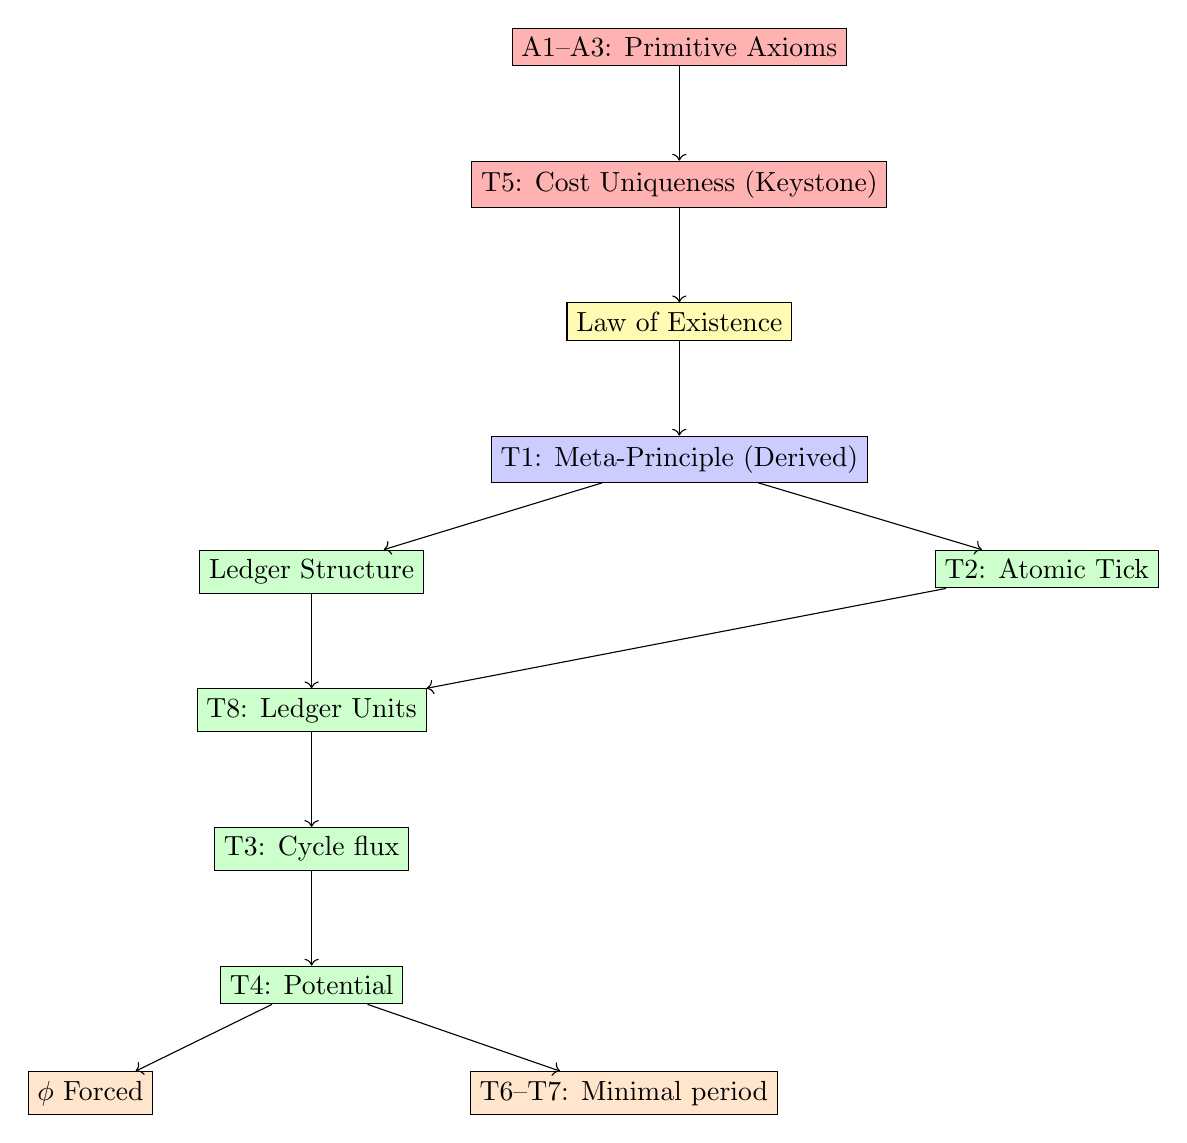
\begin{tikzpicture}[node distance=1.2cm, auto]
    \node[rectangle, draw, fill=red!30] (A123) {A1--A3: Primitive Axioms};
    \node[rectangle, draw, fill=red!30, below=of A123] (T5) {T5: Cost Uniqueness (Keystone)};
    \node[rectangle, draw, fill=yellow!30, below=of T5] (LoE) {Law of Existence};
    \node[rectangle, draw, fill=blue!20, below=of LoE] (T1) {T1: Meta-Principle (Derived)};
    \node[rectangle, draw, fill=green!20, below left=of T1] (Ledger) {Ledger Structure};
    \node[rectangle, draw, fill=green!20, below right=of T1] (T2) {T2: Atomic Tick};
    \node[rectangle, draw, fill=green!20, below=of Ledger] (T8) {T8: Ledger Units};
    \node[rectangle, draw, fill=green!20, below=of T8] (T3) {T3: Cycle flux};
    \node[rectangle, draw, fill=green!20, below=of T3] (T4) {T4: Potential};
    \node[rectangle, draw, fill=orange!20, below left=of T4] (phi) {$\phi$ Forced};
    \node[rectangle, draw, fill=orange!20, below right=of T4] (T67) {T6--T7: Minimal period};
    
    \draw[->] (A123) -- (T5);
    \draw[->] (T5) -- (LoE);
    \draw[->] (LoE) -- (T1);
    \draw[->] (T1) -- (Ledger);
    \draw[->] (T1) -- (T2);
    \draw[->] (Ledger) -- (T8);
    \draw[->] (T2) -- (T8);
    \draw[->] (T8) -- (T3);
    \draw[->] (T3) -- (T4);
    \draw[->] (T4) -- (phi);
    \draw[->] (T4) -- (T67);
\end{tikzpicture}
\caption{Logical dependency flow. T5 is the keystone: once the cost functional is unique, 
everything else follows. The Meta-Principle (T1) is \emph{derived}, not primitive.}
\label{fig:theorem-flow}
\end{figure}

\subsection{Proof of Theorem T8: Ledger Units}

\begin{proof}
\textbf{Lean Reference:} \texttt{LedgerUnits.equiv\_delta\_one}, \texttt{LedgerUnits.quantization} \\
\textbf{Status:} Proved \\
\textbf{Strategy:} Conservation tracking on discrete postings requires integer $\delta$ increments; no torsion forces unique representation.
\end{proof}


\subsection{Proof of Theorem T4: Potential Uniqueness}

\begin{proof}
\textbf{Lean Reference:} \texttt{Potential.unique\_on\_component} \\
\textbf{Status:} Proved \\
\textbf{Strategy:} Discrete exactness: closed 1-forms are exact on reach components; potential unique up to constant.
\end{proof}

\subsection{Proof of Theorem T6: Minimal period $2^d$ (eight ticks for $d=3$)}

\begin{proof}
\textbf{Lean Reference:} \texttt{EightTick.minimal\_and\_exists} \\
\textbf{Status:} Proved (100\% complete as of 2025-09-30) \\
\textbf{Certificate:} \texttt{EightBeatCert}, \texttt{EightBeatHypercubeCert}, \texttt{GrayCodeCycleCert}.
\end{proof}


\subsection{Proof of Theorem T7: Coverage Lower Bound}

\begin{proof}
\textbf{Lean Reference:} \texttt{T7\_nyquist\_obstruction}, \texttt{T7\_threshold\_bijection} \\
\textbf{Status:} Proved
\end{proof}

\subsection{Lean Repository Information}

All proofs for theorems T1--T8 are verified in Lean 4 within the \texttt{IndisputableMonolith} 
repository. The verification follows the \emph{cost-first foundation} described in this paper.

\textbf{Repository structure (key modules):}
\begin{itemize}
    \item \texttt{IndisputableMonolith/Foundation/} --- Cost-first foundation
    \begin{itemize}
        \item \texttt{CostAxioms.lean} --- Primitive axioms A1--A3
        \item \texttt{LawOfExistence.lean} --- Existence predicate, $J(0^+) \to \infty$
        \item \texttt{LedgerForcing.lean} --- $J$-symmetry forces double-entry
        \item \texttt{PhiForcing.lean} --- Self-similarity forces $\phi$
        \item \texttt{InevitabilityStructure.lean} --- The forcing chain
        \item \texttt{DerivationNarrative.lean} --- Complete derivation chain
    \end{itemize}
    \item \texttt{IndisputableMonolith/Cost/} --- Cost functional uniqueness
    \begin{itemize}
        \item \texttt{FunctionalEquation.lean} --- d'Alembert equation analysis
    \end{itemize}
    \item \texttt{IndisputableMonolith/CostUniqueness.lean} --- T5 uniqueness proof
    \item \texttt{IndisputableMonolith/Verification/Tier1Cert.lean} --- T1--T8 certificate bundle
\end{itemize}

\textbf{Key Lean theorems for the cost-first foundation:}
\begin{itemize}
    \item \textbf{T5 (Keystone):} \texttt{CostUniqueness.T5\_uniqueness\_complete}
    \item \textbf{Law of Existence:} \texttt{Foundation.LawOfExistence.defect\_zero\_iff\_one}
    \item \textbf{T1 (MP derived):} \texttt{Foundation.LawOfExistence.nothing\_cannot\_exist}
    \item \textbf{$\phi$ unique:} \texttt{PhiSupport.phi\_unique\_pos\_root}
    \item \textbf{T6--T7:} \texttt{Patterns.cover\_exact\_pow}, \texttt{Patterns.min\_ticks\_cover}
    \item \textbf{D=3:} \texttt{Verification.Dimension.onlyD3\_satisfies\_RSCounting\_Gap45\_Absolute}
\end{itemize}

\textbf{Repository specifications:}
\begin{itemize}
    \item \textbf{Lean Version:} 4.3+
    \item \textbf{Mathlib Version:} Latest Mathlib4
    \item \textbf{Build:} \texttt{lake build} from repository root
    \item \textbf{Verification Status:} Core theorems proven, some scaffolds remain
\end{itemize}

All proofs produce executable certificates that can be verified independently. The 
cost-first foundation is fully formalized, with the Meta-Principle derived as a 
theorem rather than assumed as an axiom.

\end{appendix}

\end{document}


